\documentclass[border = 1cm, a4paper]{standalone}

\usepackage{tikz}
\usetikzlibrary{shapes, arrows.meta, positioning, external}

\begin{document}

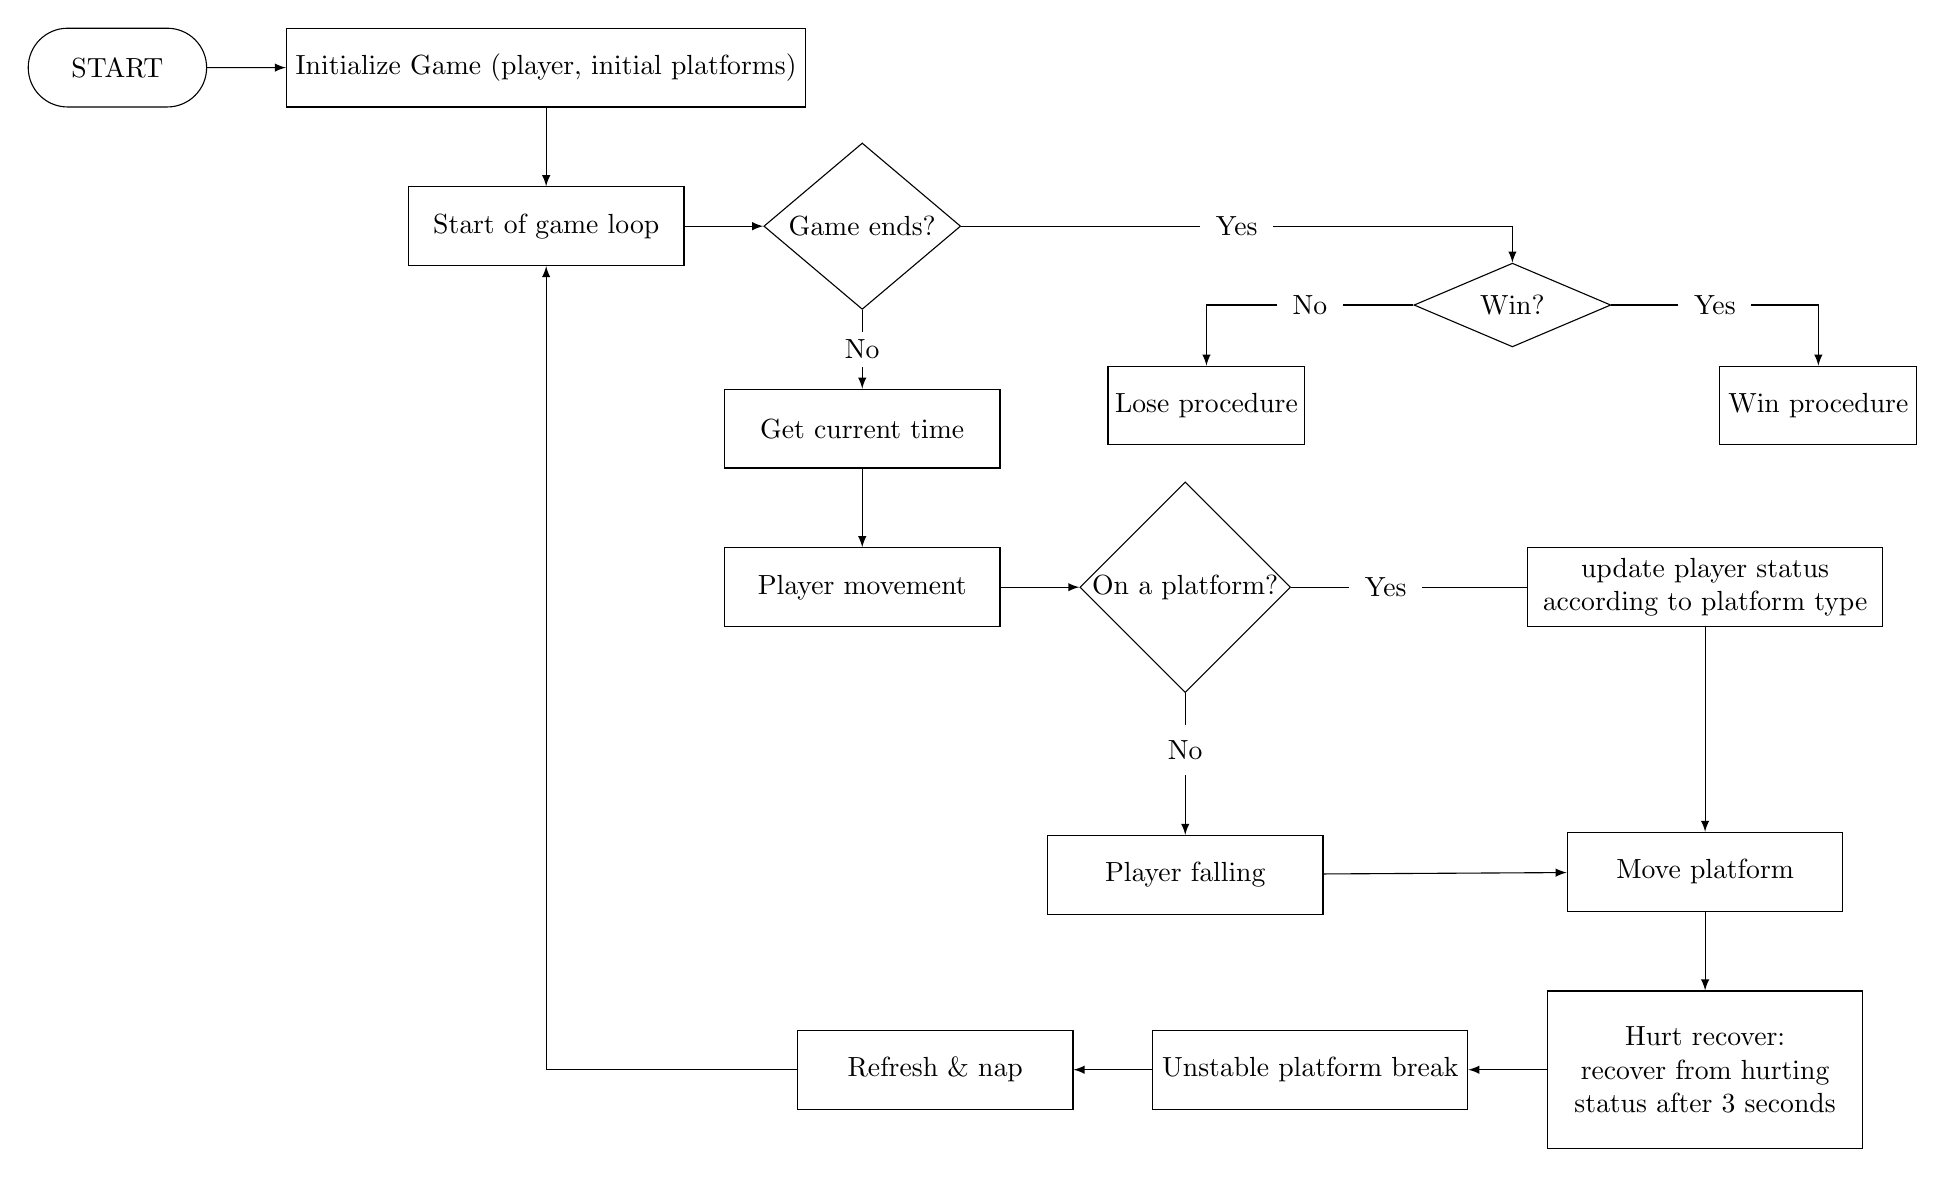
\begin{tikzpicture}

\node[draw,
    rounded rectangle,
    minimum width = 2.5cm,
    minimum height = 1cm] (start){START};

\node[draw,
    align=center,
    right=of start,
    minimum width=3.5cm,
    minimum height=1cm
] (initial) {Initialize Game (player, initial platforms)};

\node[draw,
    align = center,
    below = of initial,
    minimum width=3.5cm,
    minimum height=1cm,
    inner sep=0] (Game_loop) {Start of game loop};

\node[draw,
    diamond,
    right=of Game_loop,
    minimum width=2.5cm,
    inner sep=0] (mainloop) {Game ends?};

\node[draw,
    align = center,
    below =of mainloop,
    minimum width=3.5cm,
    minimum height=1cm,
    inner sep=0] (get_time) {Get current time};
    
\node[draw,
    align = center,
    below = of get_time,
    minimum width=3.5cm,
    minimum height=1cm,
    inner sep=0] (player) {Player movement};

\node[draw,
    diamond,
    right= of player,
    inner sep=0] (On) {On a platform?};

\node[draw,
    align = center,
    below = 1.8cm of On,
    minimum width=3.5cm,
    minimum height=1cm,
    inner sep=0] (fall) {Player falling};

\node[draw,
    align = center,
    right = 3cm of On,
    minimum width=4.5cm,
    minimum height=1cm,
    inner sep=0] (mv_lf) {update player status \\
                            according to platform type};

\node[draw,
    align = center,
    below =  2.6cm of mv_lf,
    minimum width=3.5cm,
    minimum height=1cm,
    inner sep=0] (platform) {Move platform};

\node[draw,
    align = center,
    below = of platform,
    minimum width=4.0cm,
    minimum height=2cm,
    inner sep=0] (hurtR) {Hurt recover: \\
                        recover from hurting \\
                        status after 3 seconds};

\node[draw,
    align = center,
    left = of hurtR,
    minimum width=4.0cm,
    minimum height=1cm,
    inner sep=0] (UsPB) {Unstable platform break};
    
\node[draw,
    align = center,
    left = of UsPB,
    minimum width=3.5cm,
    minimum height=1cm,
    inner sep=0] (nap) {Refresh \& nap};

\node[draw,
    diamond,
    below right=0.2 cm and 7cm of mainloop,
    minimum width=2.5cm,
    inner sep=0] (check) {Win?};

\node[draw,
    align = center,
    below right = 0.5 cm and 2cm of check,
    minimum width=2.5cm,
    minimum height=1cm,
    inner sep=0] (win) {Win procedure};

\node[draw,
    align = center,
    below left = 0.5 cm and 2cm of check,
    minimum width=2.5cm,
    minimum height=1cm,
    inner sep=0] (lose) {Lose procedure};

\draw[-latex] (start) edge (initial)
    (initial) edge (Game_loop)
    (Game_loop) edge (mainloop)
    (get_time) edge (player)
    (player) edge (On)
    (On) -- (mv_lf) node[pos=0.4,fill=white,inner sep=0.2cm]{Yes}
    (On) -- (fall) node[pos=0.4,fill=white,inner sep=0.2cm]{No}
    (mv_lf) edge (platform)
    (fall) edge (platform)
    (platform) edge (hurtR)
    (hurtR) edge (UsPB)
    (UsPB) edge (nap);
\draw[-latex] (check) -| (win)
	node[pos=0.25,fill=white,inner sep=0.2cm]{Yes};
\draw[-latex] (check) -| (lose)
	node[pos=0.25,fill=white,inner sep=0.2cm]{No};
\draw[-latex] (mainloop) -| (check)
    node[pos=0.25,fill=white,inner sep=0.2cm]{Yes};
\draw[-latex] (mainloop) -- (get_time)
    node[pos=0.5,fill=white,inner sep=0.1cm]{No};
\draw[-latex] (nap) -| (Game_loop);
 
\end{tikzpicture}


\end{document}
